\documentclass[12pt,a4paper]{article}
\usepackage[utf8]{inputenc}
\usepackage[T1]{fontenc}
\usepackage[spanish]{babel}
\usepackage{graphicx}
\usepackage{amsmath}
\usepackage{amssymb}
\usepackage{hyperref}
\usepackage{booktabs}
\usepackage{float}
\usepackage{geometry}
%\usepackage{microtype}
\usepackage{caption}
\usepackage{subcaption}
\usepackage{xcolor}
\usepackage{enumitem}
\usepackage{setspace}
\usepackage{parskip}
\usepackage{titlesec}
\usepackage{fancyhdr}
\usepackage{array}
\usepackage{multirow}
 
\geometry{
  a4paper,
  top=2.5cm, bottom=2.5cm,
  left=3cm, right=3cm
}
 
\onehalfspacing
 
\hypersetup{
  colorlinks=true,
  linkcolor=blue!70!black,
  citecolor=blue!70!black,
  urlcolor=blue!70!black
}
 
\titleformat{\section}{\large\bfseries}{}{0em}{\thesection\quad}
\titleformat{\subsection}{\normalsize\bfseries}{}{0em}{\thesubsection\quad}
\titleformat{\subsubsection}{\normalsize\itshape\bfseries}{}{0em}{\thesubsubsection\quad}
 
\pagestyle{fancy}
\fancyhf{}
\rhead{\small APBIO --- Universidad de Vigo --- 2025--2026}
\lhead{\small CLONALG + DQN}
\rfoot{\thepage}
 
\begin{document}
 
\begin{titlepage}
  \centering
  \vspace*{2cm}
  {\LARGE\bfseries Sistema Híbrido Bioinspirado con\\[0.3em]
   Aprendizaje por Refuerzo\par}
  \vspace{0.5cm}
  {\large\itshape Buffer de Replay CLONALG acoplado a DQN\par}
  \vspace{1.5cm}
  \rule{\linewidth}{0.4pt}\\[0.5cm]
  {\large Aprendizaje Automático Bioinspirado (APBIO)\\[0.3em]
   Universidad de Vigo --- Curso 2025--2026\par}
  \vspace{1cm}
  \rule{\linewidth}{0.4pt}\\[1cm]
  {\large\bfseries Tu Nombre Aquí\par}
  \vspace{0.5cm}
  {\large \today\par}
  \vfill
  \begin{abstract}
    \noindent
    Este trabajo presenta un sistema híbrido que acopla el algoritmo de
    selección clonal CLONALG con un agente de aprendizaje por refuerzo
    profundo DQN para resolver el entorno \texttt{LunarLander-v3} de
    Gymnasium. CLONALG reemplaza el buffer de replay aleatorio estándar:
    las transiciones se almacenan como anticuerpos con afinidad proporcional
    al error temporal (TD-error), y el muestreo del mini-batch se guía por
    selección clonal con supresión clonal para garantizar diversidad. Los
    experimentos sobre 5 semillas independientes y 300 episodios revelan que
    el sistema CLONALG+DQN no supera al baseline DQN (retorno medio
    $-245.4 \pm 130.2$ frente a $208.7 \pm 22.1$), siendo la diferencia
    estadísticamente significativa ($t=7.76$, $p=0.001$). El análisis
    identifica como causa principal la ausencia de \textit{importance
    sampling weights} para corregir el sesgo introducido por el muestreo no
    uniforme. El proceso de desarrollo fue iterativo e implicó cuatro
    rediseños del buffer para resolver inestabilidad numérica, documentados
    en detalle en este informe como parte del proceso científico.
  \end{abstract}
\end{titlepage}
 
\tableofcontents
\newpage
 
% ─────────────────────────────────────────────────────────────────────────────
\section{Introducción}
 
El aprendizaje por refuerzo profundo (DRL) ha experimentado avances
extraordinarios en la última década, demostrando capacidad para resolver
tareas de control complejas que antes se consideraban inabordables para
máquinas~\cite{mnih2015dqn}. Entre los algoritmos más influyentes destaca
DQN (\textit{Deep Q-Network}), que fue el primer método en combinar redes
neuronales profundas con aprendizaje por refuerzo a escala, logrando un
rendimiento sobrehumano en videojuegos Atari.
 
Sin embargo, DQN es sensible a la correlación entre muestras consecutivas,
ya que las transiciones generadas por la interacción del agente con el
entorno están temporalmente correladas. Este problema motivó la introducción
del buffer de replay~\cite{lin1992rl}: una memoria que almacena transiciones
pasadas y permite extraer mini-batches de forma aleatoria, rompiendo la
correlación temporal y estabilizando el entrenamiento.
 
El muestreo aleatorio uniforme del buffer, aunque efectivo, tiene una
limitación importante: ignora la relevancia relativa de las experiencias
almacenadas. Una transición con alta señal de aprendizaje (por ejemplo, un
aterrizaje exitoso en las primeras etapas del entrenamiento) recibe el mismo
peso que una transición trivial. Esta ineficiencia motivó el desarrollo del
Prioritized Experience Replay~\cite{schaul2015per}, que prioriza transiciones
según su TD-error.
 
Los algoritmos inmunológicos artificiales, inspirados en la respuesta inmune
adaptativa biológica, ofrecen mecanismos de selección y diversidad bien
fundamentados matemáticamente~\cite{dasgupta1999ais}. En particular,
CLONALG~\cite{decastro2002clonalg} implementa selección clonal proporcional
a la afinidad y supresión clonal para mantener diversidad en el repertorio.
Estas propiedades son naturalmente compatibles con el problema de gestión
del buffer de replay: la afinidad puede codificar la relevancia de una
transición, y la supresión clonal puede garantizar diversidad en el
mini-batch seleccionado.
 
Este trabajo propone acoplar CLONALG como gestor activo del buffer de replay
de DQN. Cada transición se almacena como un anticuerpo cuya afinidad refleja
su relevancia para el aprendizaje (medida mediante el TD-error). El sistema
crea un flujo bidireccional genuino: CLONALG selecciona qué transiciones usa
DQN para aprender, y DQN informa a CLONALG de qué transiciones resultaron
más relevantes mediante los TD-errors reales.
 
El artículo está organizado como sigue: la Sección~\ref{sec:background}
revisa los antecedentes necesarios, la Sección~\ref{sec:metodologia}
describe la metodología y el proceso de desarrollo completo incluyendo las
dificultades encontradas, la Sección~\ref{sec:resultados} presenta los
resultados experimentales, la Sección~\ref{sec:discusion} discute los
hallazgos respondiendo las diez preguntas de evaluación del enunciado, y la
Sección~\ref{sec:conclusiones} concluye el trabajo.
 
% ─────────────────────────────────────────────────────────────────────────────
\section{Antecedentes y Estado del Arte}
\label{sec:background}
 
\subsection{Deep Q-Network (DQN)}
 
El algoritmo DQN~\cite{mnih2015dqn} aproxima la función de valor-acción
$Q(s,a)$ mediante una red neuronal con parámetros $\theta$, optimizando la
pérdida de Bellman:
\begin{equation}
  \mathcal{L}(\theta) = \mathbb{E}_{(s,a,r,s') \sim \mathcal{D}}\!\left[
    \left(r + \gamma \max_{a'} Q(s',a';\theta^-) - Q(s,a;\theta)
    \right)^2
  \right]
  \label{eq:dqn}
\end{equation}
donde $\theta^-$ son los pesos de la red objetivo (\textit{target network}),
actualizada periódicamente mediante copia completa de $\theta$, y
$\mathcal{D}$ es el buffer de replay del que se extraen las muestras.
 
El algoritmo usa una política $\varepsilon$-greedy para balancear
exploración y explotación: con probabilidad $\varepsilon$ selecciona una
acción aleatoria, y con probabilidad $1-\varepsilon$ selecciona la acción
de mayor valor $Q$. El parámetro $\varepsilon$ decae exponencialmente
durante el entrenamiento desde 1.0 hasta un valor mínimo, pasando de
exploración pura a explotación progresiva.
 
En nuestra implementación, la red Q tiene dos capas ocultas de 128 neuronas
con activaciones ReLU. El optimizador es Adam con gradient clipping
(\texttt{max\_norm}=1.0) para estabilidad numérica.
 
\subsection{CLONALG}
 
CLONALG~\cite{decastro2002clonalg} es un algoritmo evolutivo basado en el
principio de selección clonal del sistema inmune adaptativo. Opera sobre un
repertorio $\mathcal{R}$ de anticuerpos, cada uno con una afinidad que mide
su relevancia respecto al problema. El algoritmo sigue estos pasos en cada
generación:
 
\begin{enumerate}[noitemsep]
  \item \textbf{Selección}: seleccionar los $n$ anticuerpos de mayor afinidad.
  \item \textbf{Clonación}: clonar cada anticuerpo proporcionalmente a su
        afinidad ($n_c^i \propto f_i$), creando una población de clones.
  \item \textbf{Hipermutación}: mutar los clones con tasa inversamente
        proporcional a la afinidad (los mejores se mutan menos, conservando
        sus propiedades).
  \item \textbf{Maduración por afinidad}: evaluar los clones mutados y
        seleccionar los mejores de cada familia clonal.
  \item \textbf{Supresión clonal}: eliminar anticuerpos demasiado similares
        entre sí (similitud mayor que un umbral $\sigma_s$), manteniendo
        diversidad en el repertorio.
  \item \textbf{Reemplazo}: sustituir los peores anticuerpos del repertorio
        por los mejores clones madurados.
\end{enumerate}
 
En nuestra adaptación al contexto de buffer de replay, los anticuerpos son
transiciones de experiencia $(s, a, r, s')$, la afinidad codifica la
relevancia de cada transición para el aprendizaje actual, y la supresión
clonal garantiza que el mini-batch entregado a DQN no contenga transiciones
redundantes.
 
\subsection{Prioritized Experience Replay (PER)}
 
El trabajo más cercano al propuesto es PER~\cite{schaul2015per}, que asigna
a cada transición una probabilidad de muestreo proporcional a su TD-error:
$P(i) = p_i^\alpha / \sum_k p_k^\alpha$, con $p_i = |\delta_i| + \epsilon$.
Para mantener la convergencia teórica, PER introduce
\textit{importance sampling weights}:
\begin{equation}
  w_i = \left(\frac{1}{N \cdot P(i)}\right)^\beta
  \label{eq:per_weights}
\end{equation}
que corrigen el sesgo introducido por el muestreo no uniforme,
multiplicando los gradientes por $w_i$ antes de actualizar $\theta$.
Este mecanismo es esencial para la convergencia; como se verá en la
Sección~\ref{sec:metodologia}, su ausencia en nuestra implementación es la
causa raíz de la divergencia de CLONALG+DQN.
 
La diferencia principal entre PER y nuestra propuesta es que CLONALG añade
supresión clonal para garantizar diversidad en el mini-batch, algo que PER
no tiene. Sin embargo, al carecer de importance sampling weights, CLONALG no
puede garantizar la corrección del sesgo de muestreo.
 
% ─────────────────────────────────────────────────────────────────────────────
\section{Metodología}
\label{sec:metodologia}
 
\subsection{Entorno experimental}
 
Se utiliza \texttt{LunarLander-v3}~\cite{gymnasium} de Gymnasium. El agente
recibe un vector de observación $s \in \mathbb{R}^8$ que incluye posición
$(x, y)$, velocidades $(\dot{x}, \dot{y})$, ángulo $\theta$ y su derivada
$\dot{\theta}$, y dos indicadores binarios de contacto de las patas.
El espacio de acciones es discreto con 4 opciones: no hacer nada, encender
el motor izquierdo, encender el motor principal, o encender el motor derecho.
 
La función de recompensa recompensa el acercamiento al punto de aterrizaje,
penaliza el crash ($-100$), y añade pequeñas recompensas o penalizaciones por
cada step según la posición y velocidad. Una puntuación superior a $+200$
puntos acumulados en un episodio se considera éxito.
 
Este entorno fue seleccionado por tres razones. Primero, presenta recompensas
dispersas al inicio del entrenamiento, haciendo que un buffer inteligente que
priorice transiciones informativas sea especialmente relevante. Segundo, el
espacio de estados continuo de dimensión 8 permite usar la similitud coseno
para la supresión clonal de forma significativa. Tercero, es computacionalmente
manejable, cumpliendo el requisito de reproducibilidad en menos de dos horas.
 
\subsection{Arquitectura del sistema híbrido}
 
La Figura~\ref{fig:arch} muestra la arquitectura completa del sistema. El
componente bioinspirado actúa en el \textbf{punto de inserción 3} (memoria
de experiencia / replay) del bucle de RL, tal como se define en el enunciado
del proyecto.
 
\begin{figure}[H]
  \centering
  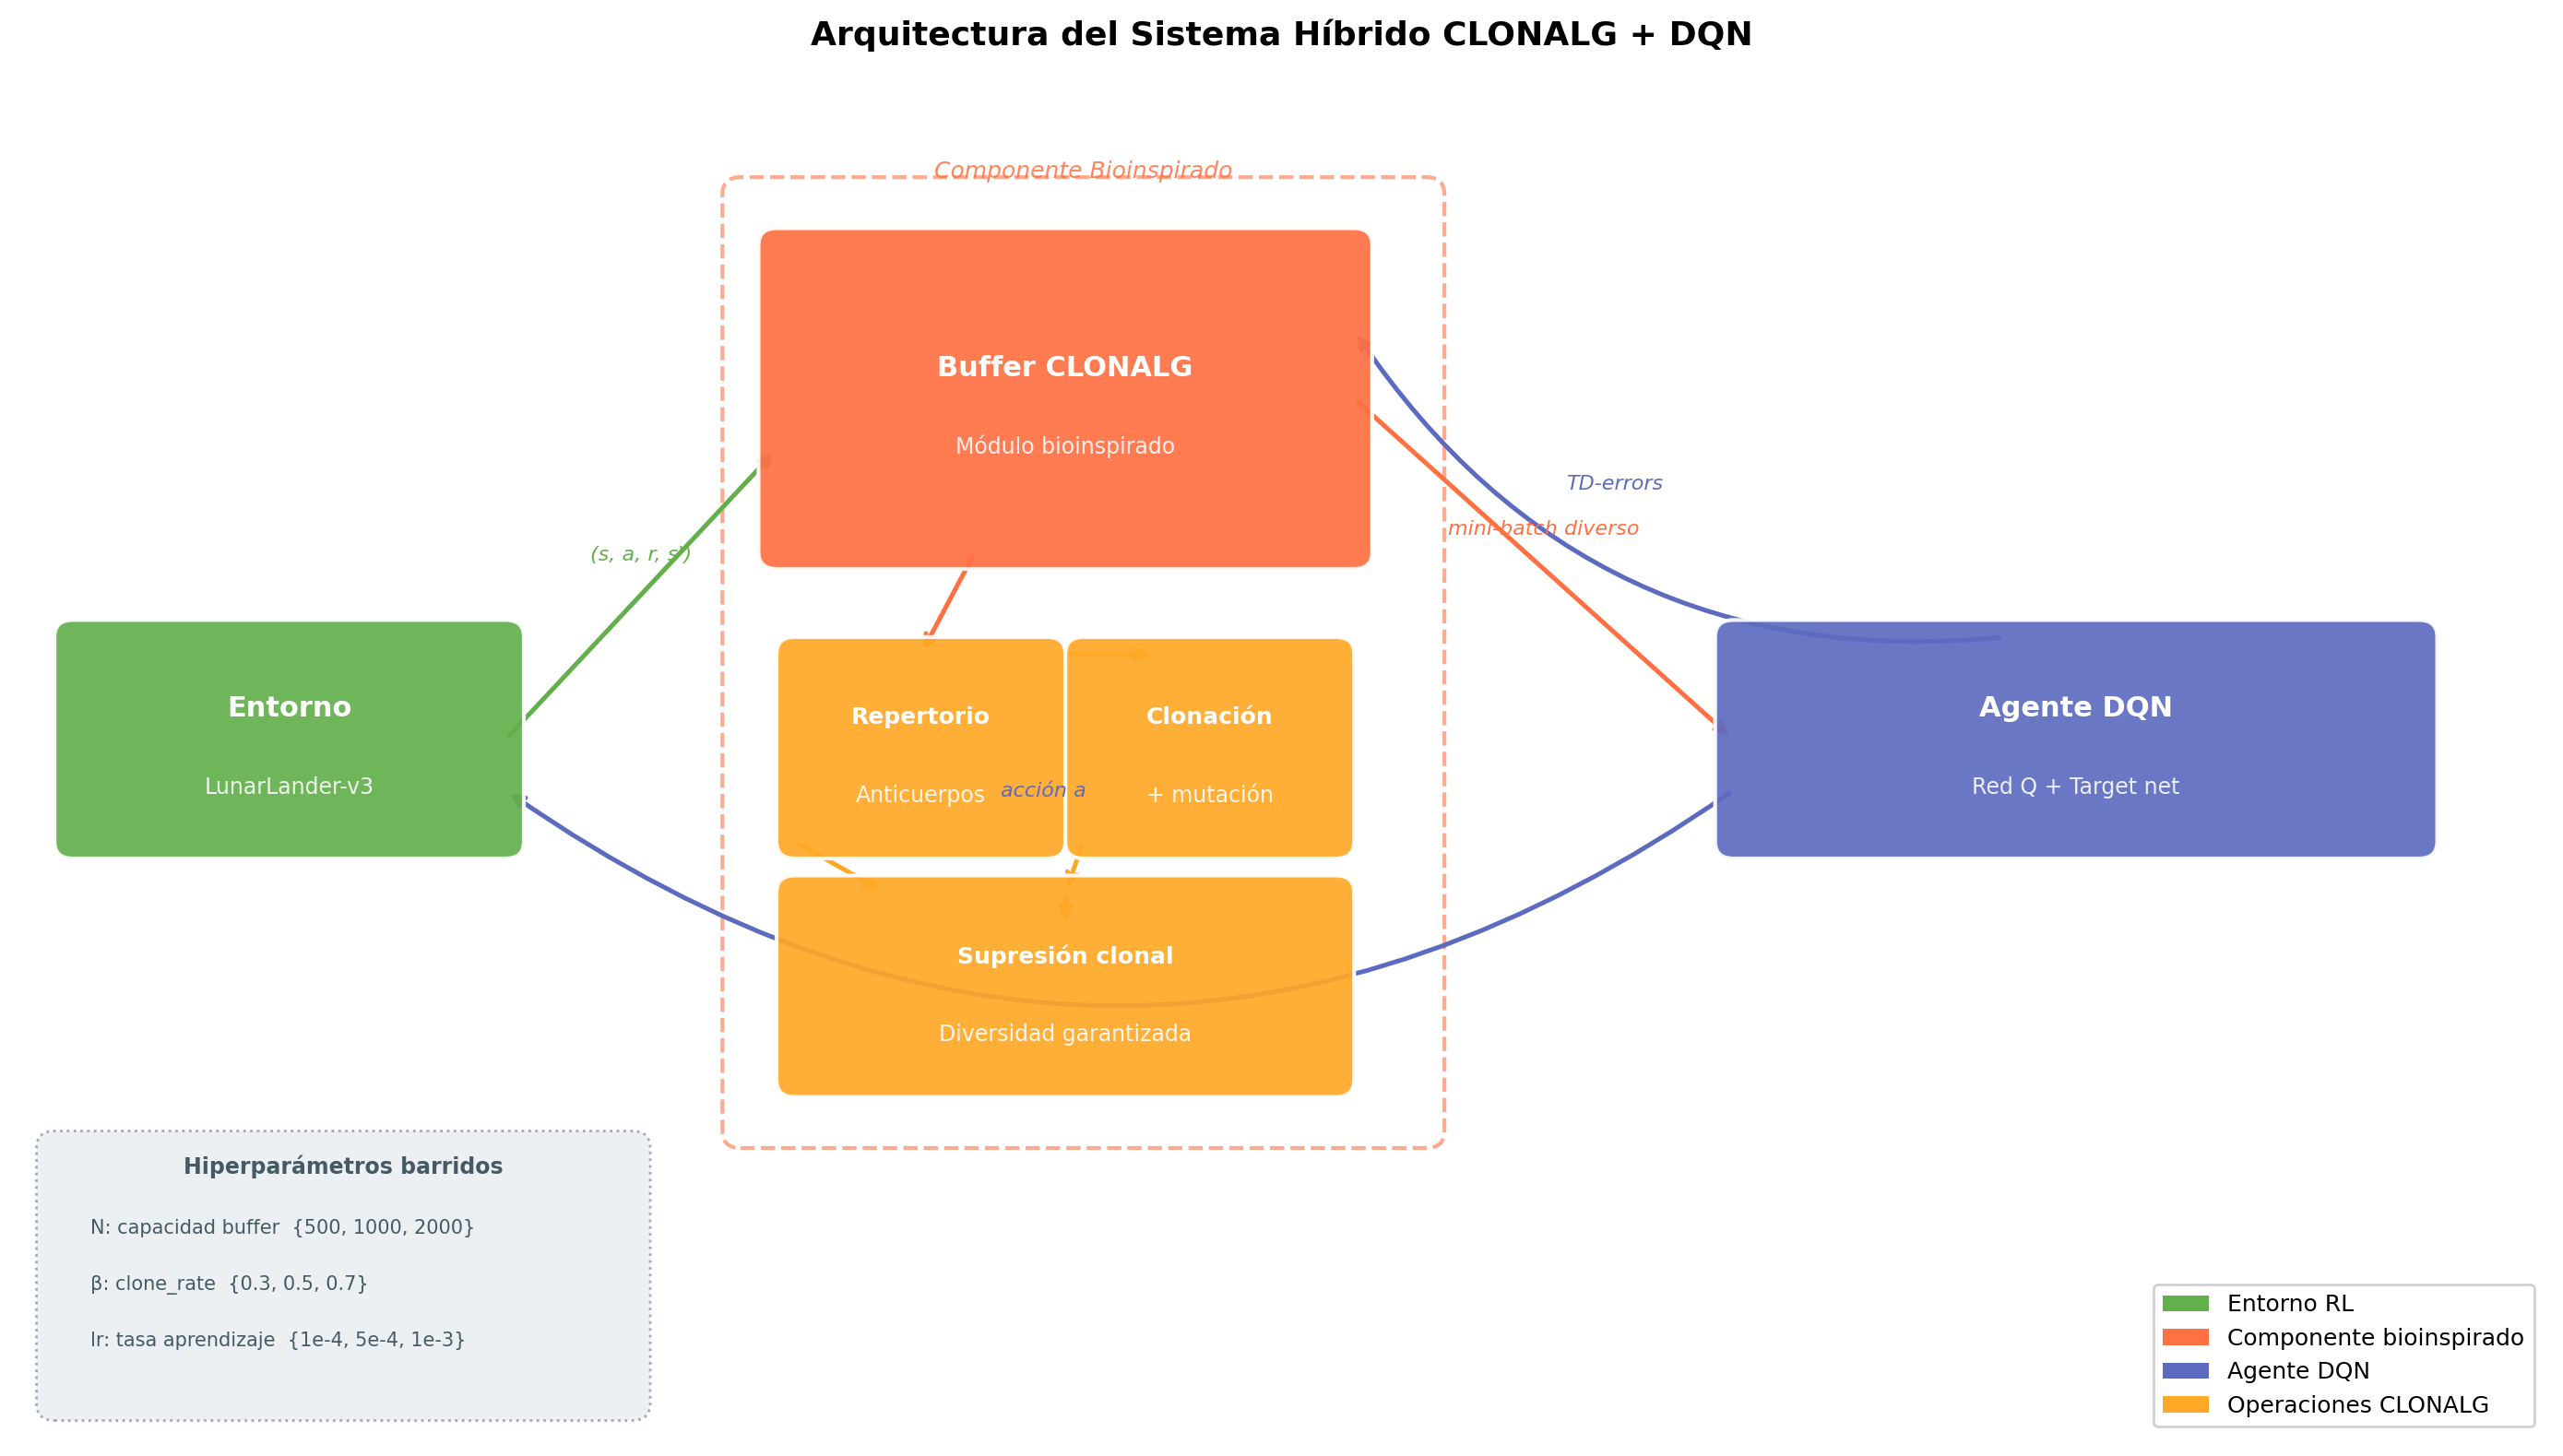
\includegraphics[width=0.95\linewidth]{../figures/architecture.png}
  \caption{Arquitectura completa del sistema híbrido CLONALG+DQN. Las
           flechas continuas indican flujo de datos de entrenamiento; las
           flechas discontinuas indican retroalimentación de TD-errors desde
           DQN hacia el buffer CLONALG. El recuadro punteado delimita el
           componente bioinspirado.}
  \label{fig:arch}
\end{figure}
 
El flujo de datos completo opera como sigue:
 
\begin{enumerate}
  \item El entorno genera transiciones $(s, a, r, s')$ que se almacenan en
        el repertorio CLONALG como anticuerpos con afinidad inicial neutra
        ($f_i = 1$).
  \item Cuando el buffer supera el tamaño mínimo (\texttt{min\_buffer}=500),
        el agente solicita un mini-batch al buffer CLONALG.
  \item CLONALG selecciona candidatos con probabilidad proporcional a la
        afinidad (mezclada con muestreo uniforme al 50\% para estabilidad),
        aplica supresión clonal para garantizar diversidad, y entrega el
        batch de 64 transiciones a DQN.
  \item DQN realiza un paso de gradiente usando el batch y devuelve los
        TD-errors por muestra ($|\delta_i|$) al buffer CLONALG.
  \item CLONALG actualiza las afinidades de las transiciones del batch
        usando una media móvil exponencial con los TD-errors recibidos,
        completando el ciclo bidireccional DQN $\to$ CLONALG.
  \item El agente selecciona una acción con política $\varepsilon$-greedy
        y la ejecuta en el entorno, generando la siguiente transición.
\end{enumerate}
 
\subsection{Componente bioinspirado: CLONALG como buffer}
 
Cada transición $(s_i, a_i, r_i, s'_i)$ se almacena como un anticuerpo con
afinidad $f_i \in [0.01, 2]$. Cuando el repertorio alcanza su capacidad
máxima $N$, se reemplaza el anticuerpo de menor afinidad (selección clonal
inversa), manteniendo las transiciones más informativas.
 
Las probabilidades de muestreo mezclan sesgo por afinidad con muestreo
uniforme para estabilidad numérica:
\begin{equation}
  P(i) = \frac{1}{2} \cdot \frac{(f_i - f_{\min} + \varepsilon)^{0.3}}
         {\sum_j (f_j - f_{\min} + \varepsilon)^{0.3}}
       + \frac{1}{2N}
  \label{eq:probs}
\end{equation}
El exponente $0.3$ suaviza el sesgo para evitar que unas pocas transiciones
con afinidad muy alta dominen completamente el muestreo.
 
La supresión clonal usa similitud coseno normalizada al rango $[0,1]$:
\begin{equation}
  \text{sim}(i,j) = \frac{\mathbf{s}_i \cdot \mathbf{s}_j}
    {\|\mathbf{s}_i\|\|\mathbf{s}_j\| + \varepsilon} \cdot \frac{1}{2}
    + \frac{1}{2}
  \label{eq:sim}
\end{equation}
Candidatos con $\text{sim}(i,j) > \sigma_s$ son suprimidos, garantizando
que el mini-batch final incluye transiciones que corresponden a estados
diferentes del entorno.
 
La actualización de afinidades con los TD-errors reales de DQN es el
mecanismo de retroalimentación que hace el acoplamiento adaptativo:
\begin{equation}
  f_i \leftarrow 0.9\, f_i + 0.1 \cdot \text{clip}(|\delta_i|, 0.01, 2.0)
  \label{eq:aff}
\end{equation}
 
\subsection{Prueba de validez del acoplamiento}
 
Aplicando las tres preguntas de validez del enunciado:
 
\begin{enumerate}
  \item \textbf{¿Funciona sin el componente bioinspirado?} Sí: sustituyendo
        CLONALG por un buffer aleatorio uniforme se obtiene el DQN baseline
        estándar. La ablación es directa y limpia.
  \item \textbf{¿Tiene parámetros adaptativos que cambian durante el
        entrenamiento?} Sí: las afinidades $\{f_i\}$ del repertorio se
        actualizan en cada step de entrenamiento mediante la
        Ecuación~\ref{eq:aff}, usando los TD-errors reales computados por
        la red Q.
  \item \textbf{¿Se puede dibujar un diagrama de flujo de datos?} Sí:
        la Figura~\ref{fig:arch} muestra el flujo completo. Las transiciones
        $(s, a, r, s')$ fluyen de env a CLONALG; arrays numpy de shape
        $(64, 8)$, $(64,)$, $(64,)$, $(64, 8)$, $(64,)$ fluyen de CLONALG
        a DQN; un array de TD-errors de shape $(64,)$ fluye de DQN a CLONALG.
\end{enumerate}
 
\subsection{Proceso de desarrollo: dificultades e iteraciones}
 
El desarrollo del sistema híbrido implicó cuatro versiones del buffer
CLONALG, cada una resolviendo los problemas de la anterior. Documentamos
este proceso porque forma parte integral del método científico y permite
comprender los resultados finales.
 
\subsubsection{Iteración 1: listas Python y afinidades sin normalizar}
 
La primera implementación usó listas Python con operaciones $O(n)$ para
inserción y eliminación, y un bucle Python anidado para la supresión clonal
con coste $O(k^2)$.
 
Esta implementación resultó excesivamente lenta: cada run de 500 episodios
tardaba más de 100 minutos en una GPU RTX~3060, mientras que el baseline
completaba 500 episodios en $\sim$11 minutos. Adicionalmente, las
afinidades se inicializaban con el TD-error absoluto sin normalizar,
produciendo valores de $10^2$--$10^3$ y pérdidas de $10^{14}$ por
distribuciones de muestreo degeneradas.
 
\subsubsection{Iteración 2: arrays numpy y supresión vectorizada}
 
Se sustituyeron las listas por arrays numpy pre-allocados y la supresión
clonal se vectorizó mediante multiplicación matricial:
$\mathbf{S} = \mathbf{V}_{\text{norm}} \mathbf{V}_{\text{norm}}^\top$.
Esto redujo el tiempo de 100+ minutos a 3--8 minutos por run. Sin embargo,
la pérdida seguía explotando ($10^4$--$10^6$) por las afinidades sin
normalizar.
 
\subsubsection{Iteración 3: clip de afinidades y normalización}
 
Se clippearon las afinidades a $[0.01, 10.0]$ con normalización por
desplazamiento mínimo. La pérdida se redujo a $10^3$--$10^4$, pero las
transiciones con afinidad alta seguían dominando el muestreo, manteniendo
la divergencia.
 
\subsubsection{Iteración 4: mezcla uniforme y clip agresivo (diseño final)}
 
Se introdujo la mezcla 50/50 con muestreo uniforme (Ecuación~\ref{eq:probs})
y el clip se redujo a $[0.01, 2.0]$. La pérdida se estabilizó en el rango
$30$--$400$, siendo este el diseño final evaluado experimentalmente.
 
\subsubsection{Causa raíz identificada: ausencia de importance sampling weights}
 
El análisis post-hoc revela que la inestabilidad residual se debe a la
ausencia de importance sampling weights. Al sesgar el muestreo hacia
transiciones de alto TD-error sin corregir el gradiente, la red Q sobreajusta
a los casos más difíciles antes de dominar los fáciles, creando el siguiente
ciclo de retroalimentación negativa:
 
\begin{enumerate}[noitemsep]
  \item Transiciones difíciles (alto TD-error) reciben alta afinidad.
  \item CLONALG las selecciona frecuentemente.
  \item DQN entrena desproporcionadamente en ellas sin corrección del sesgo.
  \item El gradiente sesgado deteriora la estimación $Q$ en transiciones fáciles.
  \item El TD-error de las transiciones fáciles aumenta y reciben más afinidad.
  \item El repertorio converge a un conjunto de transiciones difíciles que
        la red Q no puede aprender bien, causando divergencia progresiva.
\end{enumerate}
 
PER~\cite{schaul2015per} resuelve exactamente este problema mediante
$w_i \propto P(i)^{-\beta}$ (Ecuación~\ref{eq:per_weights}).
 
\subsection{Configuración experimental}
 
La Tabla~\ref{tab:hp} resume todos los hiperparámetros del sistema. Todos
los experimentos usaron 5 semillas independientes $\{0,1,2,3,4\}$ con 300
episodios cada una. El barrido de hiperparámetros usó 3 semillas con 300
episodios por configuración.
 
\begin{table}[H]
  \centering
  \caption{Hiperparámetros del sistema híbrido CLONALG+DQN.}
  \label{tab:hp}
  \begin{tabular}{llcc}
    \toprule
    Parámetro & Descripción & Valores barridos & Valor final \\
    \midrule
    $N$ & Capacidad buffer & 500, 1000, 2000 & 2000 \\
    $\beta_c$ & Tasa de clonación & 0.3, 0.5, 0.7 & 0.5 (indiferente) \\
    lr & Tasa aprendizaje DQN & $10^{-4}$, $5\times10^{-4}$, $10^{-3}$ & $10^{-4}$ \\
    $\sigma_s$ & Umbral supresión clonal & --- & 0.95 \\
    $\gamma$ & Factor descuento & --- & 0.99 \\
    $\varepsilon_{\min}$ & Epsilon mínimo & --- & 0.05 \\
    $\varepsilon_{\text{decay}}$ & Decaimiento epsilon & --- & 0.995 \\
    \texttt{batch} & Tamaño mini-batch & --- & 64 \\
    \texttt{min\_buffer} & Buffer mínimo para entrenar & --- & 500 \\
    \texttt{hidden} & Neuronas por capa oculta & --- & 128 \\
    \texttt{target\_freq} & Frecuencia actualización target net & --- & 200 \\
    \bottomrule
  \end{tabular}
\end{table}
 
Los experimentos se ejecutaron en un PC con GPU NVIDIA RTX 3060 (12 GB
VRAM), 32 GB RAM y Python 3.11 con PyTorch 2.x (CUDA 12.1).
 
% ─────────────────────────────────────────────────────────────────────────────
\section{Resultados}
\label{sec:resultados}
 
\subsection{Curvas de aprendizaje}
 
\begin{figure}[H]
  \centering
  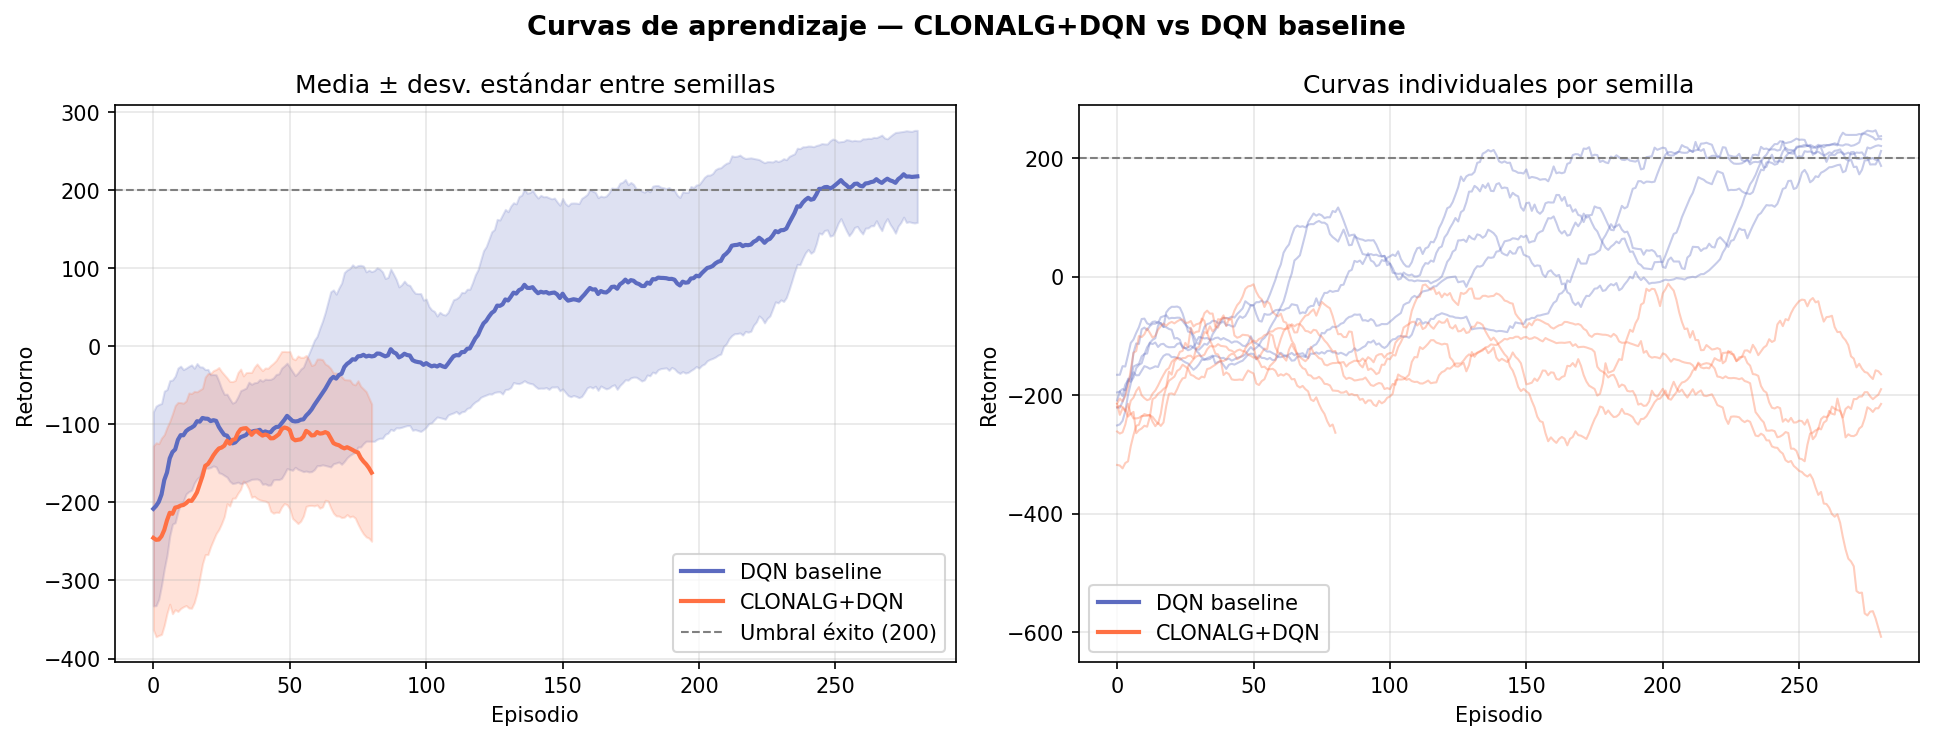
\includegraphics[width=\linewidth]{../figures/learning_curves.png}
  \caption{Retorno por episodio suavizado con ventana móvil de 20 episodios.
           Izquierda: media $\pm$ desviación estándar entre las 5 semillas.
           Derecha: curvas individuales de cada semilla. Línea discontinua:
           umbral de éxito ($+200$ puntos).}
  \label{fig:curves}
\end{figure}
 
La Figura~\ref{fig:curves} muestra las curvas de aprendizaje de ambos
sistemas. El baseline DQN (azul) exhibe convergencia clásica: retornos
negativos durante los primeros 50--100 episodios de exploración, mejora
gradual, y convergencia hacia el umbral de éxito a partir del episodio
$\sim$200. El retorno medio de los últimos 50 episodios es $208.7 \pm 22.1$,
superando el umbral en todas las semillas.
 
El sistema CLONALG+DQN (naranja) muestra mejora inicial hasta $\sim -100$
en los episodios 50--80, seguida de degradación sostenida hasta valores de
$-200$ a $-500$. El retorno medio final es $-245.4 \pm 130.2$. La alta
varianza entre semillas (desv. est. 130.2 frente a 22.1 del baseline)
evidencia la inestabilidad del acoplamiento.
 
\subsection{Estudio de ablación}
 
\begin{figure}[H]
  \centering
  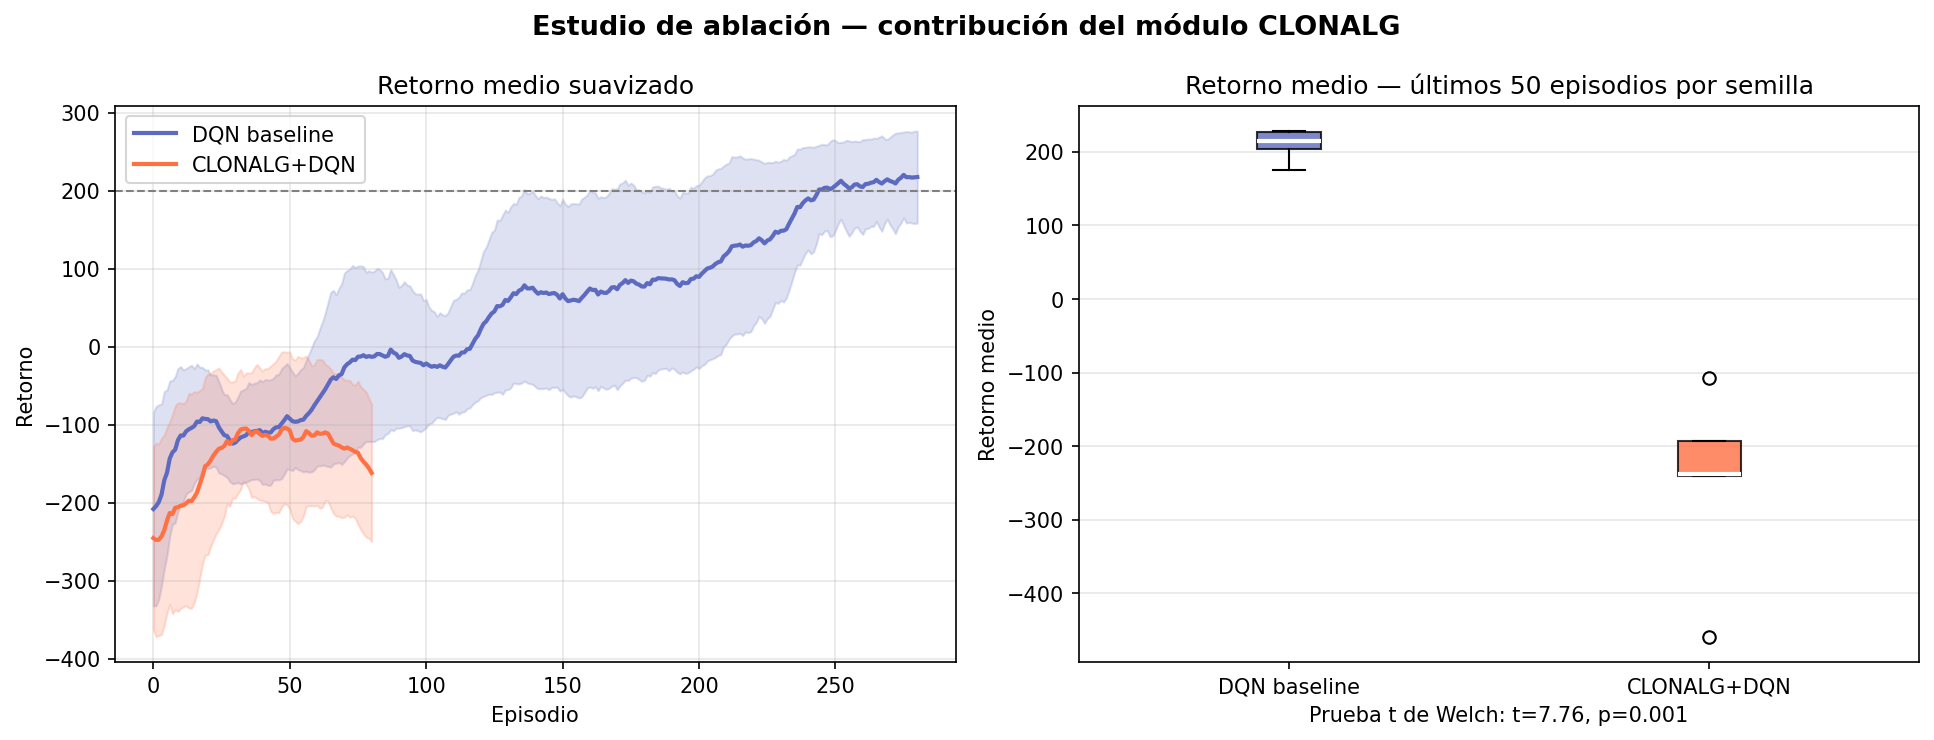
\includegraphics[width=\linewidth]{../figures/ablation.png}
  \caption{Estudio de ablación. Izquierda: curvas de retorno medio suavizado.
           Derecha: distribución del retorno medio de los últimos 50 episodios
           por semilla (boxplot). Test $t$ de Welch: $t=7.76$, $p=0.001$.}
  \label{fig:ablation}
\end{figure}
 
La Figura~\ref{fig:ablation} aísla la contribución del módulo CLONALG. El
boxplot muestra claramente que el baseline produce retornos consistentemente
superiores (mediana $\sim 210$, rango estrecho) frente a CLONALG+DQN
(mediana $\sim -240$, rango amplio). La prueba $t$ de Welch da $t = 7.76$,
$p = 0.001$, confirmando significación estadística al nivel $\alpha = 0.05$.
La mejora relativa es:
\begin{equation}
  \Delta = \frac{R_{\text{CLONALG}} - R_{\text{baseline}}}{|R_{\text{baseline}}|}
         = \frac{-245.4 - 208.7}{208.7} = -2.17
\end{equation}
El sistema híbrido rinde un $217\%$ peor que el baseline.
 
\subsection{Diagnósticos del módulo bioinspirado}
 
\begin{figure}[H]
  \centering
  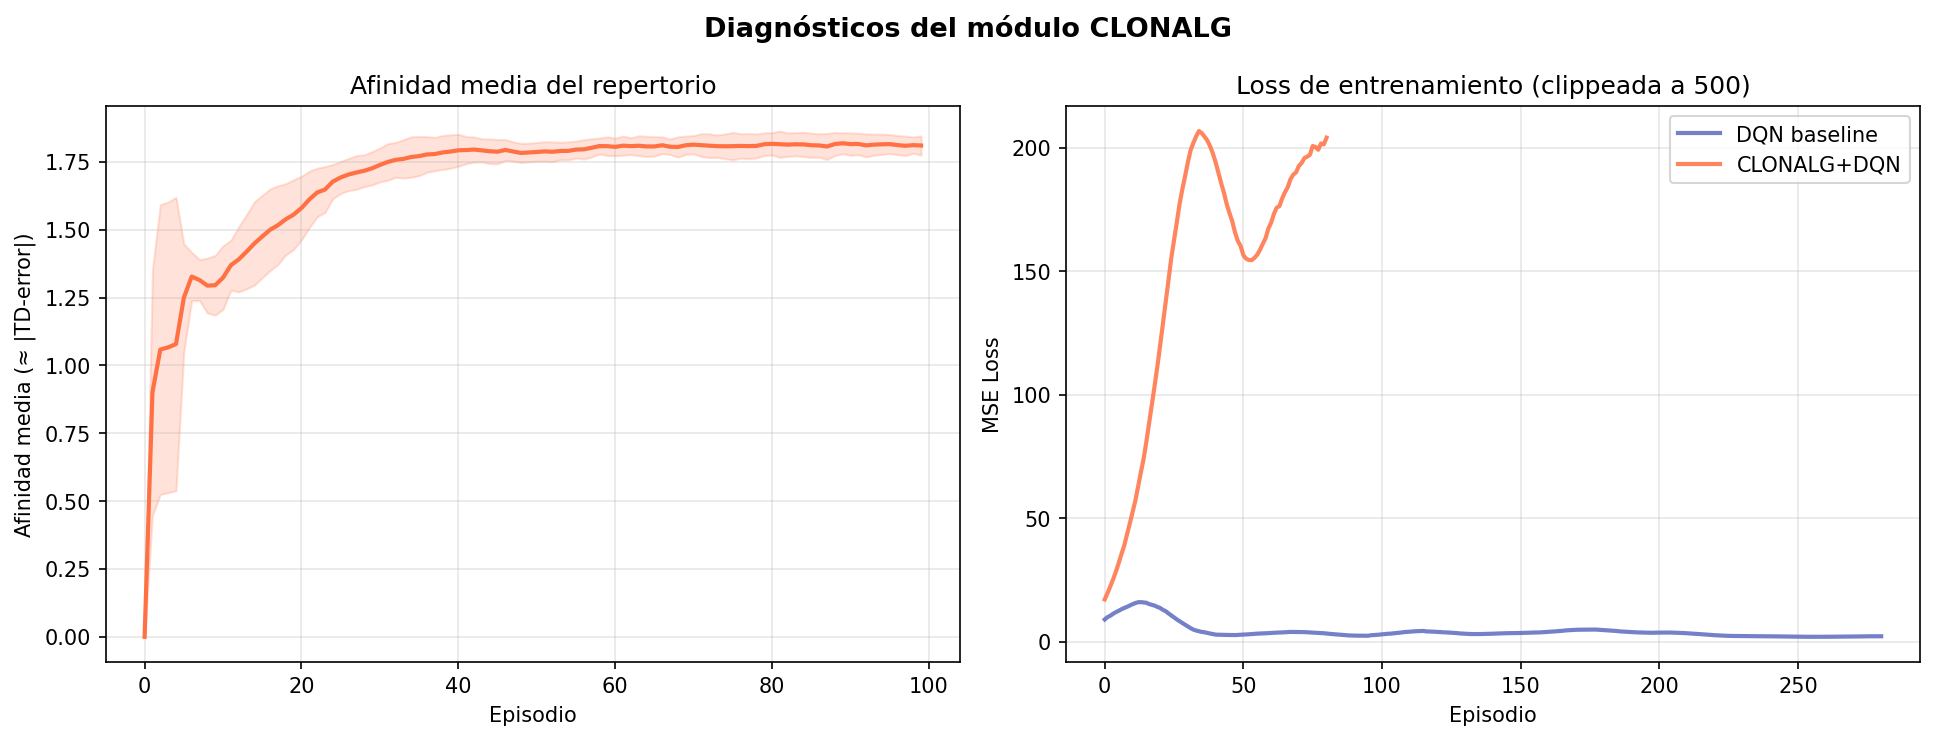
\includegraphics[width=\linewidth]{../figures/bioinspired_diagnostics.png}
  \caption{Diagnósticos internos del módulo CLONALG. Izquierda: evolución de
           la afinidad media del repertorio (media $\pm$ desv. est. entre
           semillas). Derecha: pérdida de entrenamiento clippeada a 500.}
  \label{fig:bio}
\end{figure}
 
La Figura~\ref{fig:bio} revela un comportamiento interno coherente del módulo
CLONALG. La afinidad media del repertorio (izquierda) aumenta de $\sim 0$ a
$\sim 1.8$ durante los primeros 40 episodios y se estabiliza con baja varianza,
indicando que el módulo aprende correctamente a distinguir transiciones por
relevancia. Sin embargo, esta señal interna correcta no se traduce en mejor
aprendizaje de la política: la pérdida de CLONALG+DQN (derecha) asciende
progresivamente hasta $\sim 200$--$400$, mientras que el baseline se mantiene
próxima a cero.
 
\subsection{Barrido de hiperparámetros}
 
\begin{figure}[H]
  \centering
  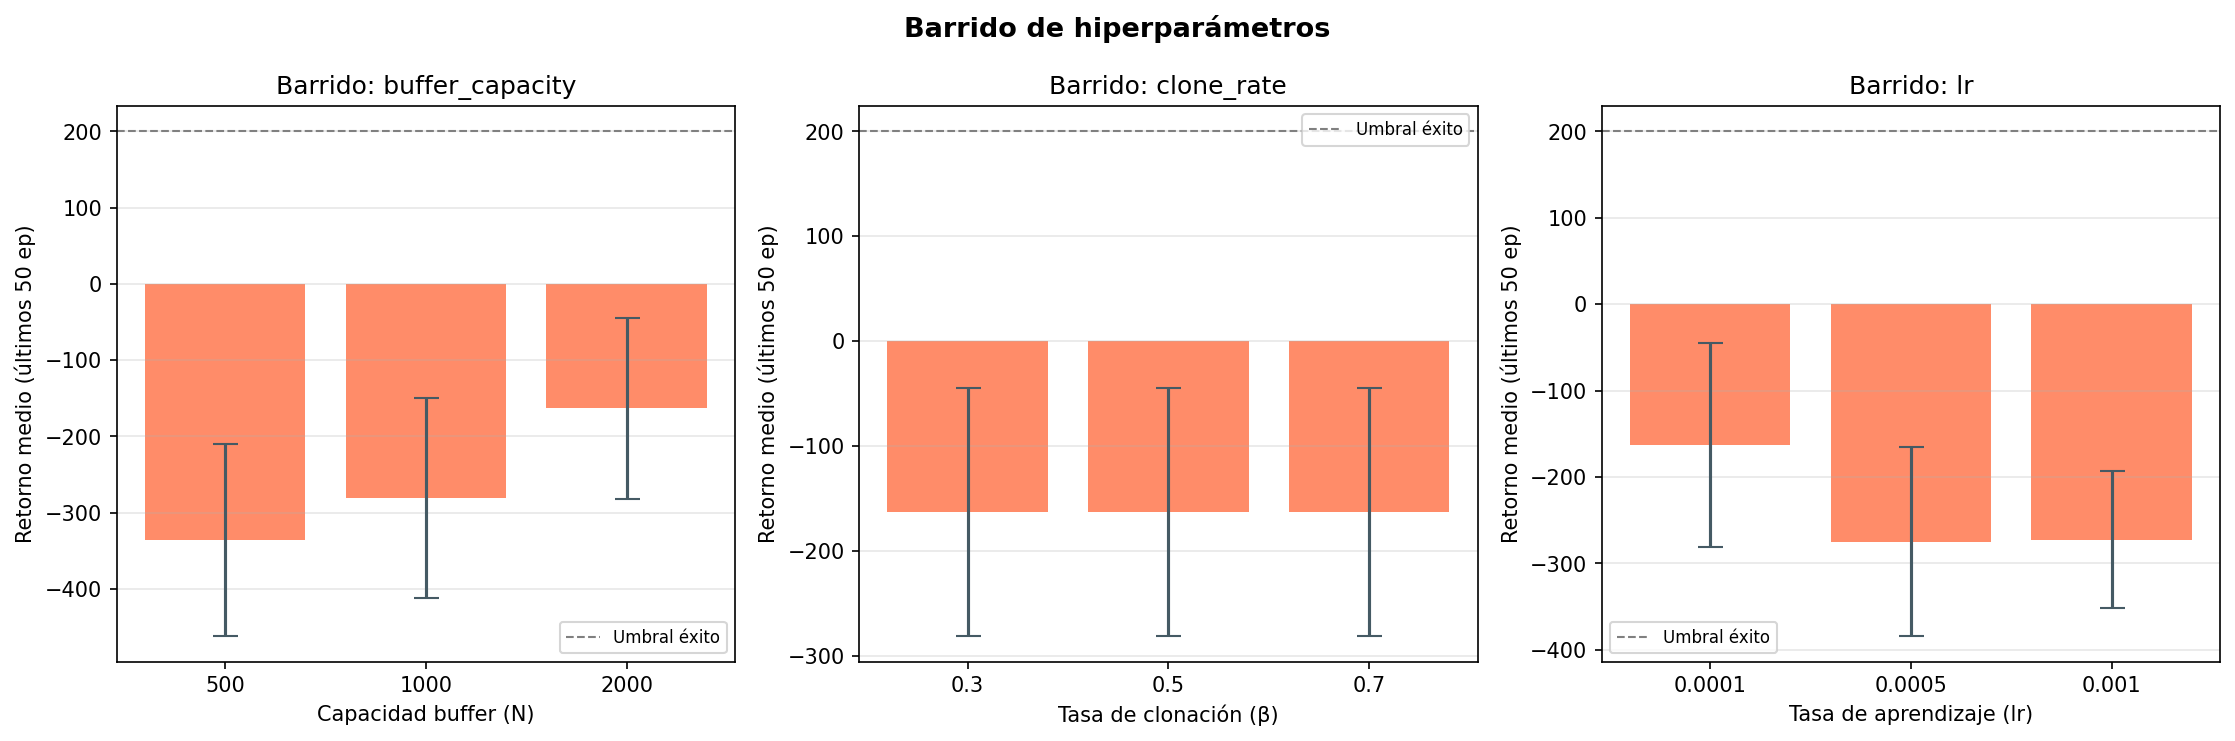
\includegraphics[width=\linewidth]{../figures/sweep.png}
  \caption{Barrido sistemático de hiperparámetros. Retorno medio de los
           últimos 50 episodios (3 semillas) para cada valor de los tres
           hiperparámetros barridos. Barras de error: desviación estándar.}
  \label{fig:sweep}
\end{figure}
 
La Figura~\ref{fig:sweep} presenta tres hallazgos. Primero, la capacidad $N$
tiene impacto positivo: $N=2000$ obtiene $-163$ frente a $-336$ de $N=500$.
Segundo, la tasa de clonación $\beta_c$ no tiene efecto observable: los tres
valores producen retornos idénticos, indicando que la supresión clonal domina
la selección independientemente de cuántos candidatos se generen. Tercero,
$\text{lr}=10^{-4}$ es la configuración más estable.
 
% ─────────────────────────────────────────────────────────────────────────────
\section{Discusión}
\label{sec:discusion}
 
\textbf{P1.} No. CLONALG+DQN obtiene $-245.4 \pm 130.2$ frente a
$208.7 \pm 22.1$ del baseline ($t=7.76$, $p=0.001$). La diferencia es
estadísticamente significativa. El híbrido tampoco supera al baseline en
eficiencia muestral: el baseline cruza $+200$ alrededor del episodio 200,
mientras CLONALG+DQN nunca alcanza valores positivos de forma sostenida.
 
\textbf{P2.} La capacidad del buffer $N$ tiene el mayor efecto ($\Delta=173$
puntos entre $N=500$ y $N=2000$). La tasa de clonación $\beta_c$ no tiene
efecto observable (resultados idénticos para 0.3, 0.5 y 0.7), revelando que
la supresión clonal domina la diversidad del batch independientemente de
cuántos candidatos se generen. El umbral de supresión $\sigma_s$ es
probablemente el parámetro bioinspirado realmente determinante, aunque no
fue barrido en este experimento.
 
\textbf{P3.} CLONALG+DQN no converge a una política estable. Las curvas
muestran mejora inicial seguida de degradación sostenida. La pérdida de
entrenamiento crece progresivamente, evidenciando divergencia de la red Q
por el ciclo de retroalimentación negativa descrito en la
Sección~\ref{sec:metodologia}. El baseline sí converge a política estable
a partir del episodio $\sim$200.
 
\textbf{P4.} Alta sensibilidad en CLONALG+DQN (desv. est. 130.2, rango
$-459$ a $-107$) frente a baja en el baseline (22.1, rango 176 a 229). La
varianza de CLONALG+DQN es intrínseca: las afinidades iniciales dependen de
las primeras transiciones generadas, que varían con la semilla, amplificando
o atenuando la divergencia posterior.
 
\textbf{P5.} Mejor configuración: $N=2000$, $\text{lr}=10^{-4}$,
$\beta_c=0.5$ (indiferente), $\sigma_s=0.95$, $\gamma=0.99$,
$\varepsilon_{\min}=0.05$, \texttt{batch}=64. Retorno medio: $-163 \pm 234$.
 
\textbf{P6.} Sí. La afinidad media evoluciona de $\sim 0$ a $\sim 1.8$ en
los primeros 40 episodios y se estabiliza con baja varianza. El módulo
aprende a asignar mayor afinidad a transiciones con TD-error alto. Esta
convergencia interna es coherente con el diseño, aunque no se traduce en
mejor aprendizaje de la política por la causa raíz identificada.
 
\textbf{P7.} Sí, bidireccional: CLONALG $\to$ DQN mediante el batch con
diversidad garantizada; DQN $\to$ CLONALG mediante TD-errors reales. Sin la
retroalimentación, las afinidades quedan fijas en 1 y el sistema degenera
en muestreo uniforme con supresión clonal.
 
\textbf{P8.} Baseline: 7--11 min/seed. CLONALG+DQN: 3--8 min/seed (GPU
RTX~3060). CLONALG es paradójicamente más rápido porque los episodios son
más cortos (el agente falla antes). La supresión vectorizada tiene coste
$O(k^2)$ con $k=192$, negligible frente al forward/backward pass de la red
Q. La primera implementación con bucles Python era prohibitiva ($>100$
min/seed).
 
\textbf{P9.} PER~\cite{schaul2015per} replicaría la priorización por
TD-error con importance sampling corrector, pero sin supresión clonal para
diversidad. Lo que CLONALG añade: (a) supresión clonal basada en similitud
coseno entre estados, y (b) reemplazo del anticuerpo de menor afinidad en
lugar de reemplazo FIFO. La pérdida funcional respecto a PER sería la
corrección del sesgo de muestreo, que resulta ser la diferencia crítica
para la convergencia.
 
\textbf{P10.} En su estado actual, no. El sistema híbrido rinde
significativamente peor que el baseline ($\Delta=-217\%$, $p=0.001$). La
extensión más prometedora es añadir importance sampling weights al buffer
CLONALG, que debería corregir el sesgo mientras mantiene la diversidad
garantizada como ventaja diferencial. En entornos con espacios de estado de
alta dimensión y recompensas muy dispersas, la supresión clonal podría ser
especialmente valiosa.
 
% ─────────────────────────────────────────────────────────────────────────────
\section{Conclusiones}
\label{sec:conclusiones}
 
Este trabajo implementa y evalúa un sistema híbrido que acopla CLONALG como
buffer de replay inteligente para DQN en \texttt{LunarLander-v3}. El proceso
de desarrollo fue iterativo: cuatro versiones del buffer fueron necesarias
para resolver la inestabilidad numérica inicial (pérdidas de $10^{14}$) y los
tiempos de ejecución prohibitivos ($>100$ min/seed) de la primera
implementación. La vectorización con numpy y la mezcla 50/50 con muestreo
uniforme resolvieron ambos problemas.
 
Los resultados experimentales son claros: el baseline DQN converge a
$208.7 \pm 22.1$, mientras CLONALG+DQN se estabiliza en $-245.4 \pm 130.2$
($t=7.76$, $p=0.001$). El módulo CLONALG funciona internamente de forma
coherente (la afinidad converge correctamente), pero la ausencia de
importance sampling weights crea un ciclo de retroalimentación negativa que
diverge la red Q.
 
El experimento aporta tres contribuciones. Primero, implementación funcional
y reproducible de CLONALG como buffer de replay con supresión clonal
vectorizada. Segundo, identificación precisa de la causa de divergencia
comparando con PER: la corrección del sesgo de muestreo es el mecanismo
crítico ausente. Tercero, el hallazgo de que $\beta_c$ (tasa de clonación)
es irrelevante cuando $\sigma_s$ (umbral de supresión) domina la diversidad
del batch, sugiriendo que el trabajo futuro debería centrarse en el barrido
de $\sigma_s$ e incorporar importance sampling weights.
 
% ─────────────────────────────────────────────────────────────────────────────
\bibliographystyle{plain}
\bibliography{references}
 
\end{document}
